\paragraph{}
The TCP/IP protocol suite provides end-to-end data communication specifying how data should be packeted, addressed, transmitted, routed and received. This functionality is organized into four abstraction layers which are used to sort all related protocols according to the scope of networking involved. From lowest to highest:
\begin{list}{}{}
\item 1. Link layer
\item 2. Internet layer
\item 3. Transport layer
\item 4. Application layer
\end{list}

\subsection{Link layer}
\paragraph{}
The link layer defines the networking methods within the scope of the local network link on which hosts communicate without intervening routers. This layer includes the protocols used to describe the local network topology and the interfaces needed to effect transmission of Internet layer datagrams to next-neighbour hosts. 
\paragraph{}
The most used protocols in this layer are studied and presented in order to find the better option for the ground segment communications.
\paragraph{}
\textbf{Ethernet}
\paragraph{}
Over the years, Ethernet, which is technically IEEE 802.3 CSMA/CD LANs, has become the most commonly used standard for enterprise networks. These networks carry voice, graphics, and video traffic.
\paragraph{}
The most common top speed is 10 gigabits per second (Gbps). With so much data being carried, the potential increases for more and more packet collisions in the collision domain. When a collision occurs, both data frames must be re-sent and this cuts down drastically 
\paragraph{}
Systems communicating over Ethernet divide a stream of data into shorter pieces called frames. Each frame contains source and destination addresses, and error-checking data so that damaged frames can be detected and discarded; most often, higher-layer protocols trigger retransmission of lost frames.
\paragraph{}
See more in \cite{Ethernet}

\paragraph{} \textbf{IEEE 802.11}
\paragraph{}
IEEE 802.11 is a set of media access control (MAC) and physical layer (PHY) specifications for implementing wireless local area network (WLAN) computer communication in the 900 MHz and 2.4, 3.6, 5, and 60 GHz frequency bands. 
\paragraph{}
With this connection the client would have a range of arround 60 m and  a data rate that can arriive to 5 Gbit/s.
\paragraph{}
See more in \cite{80211}

\paragraph{} \textbf{Frame Relay}
\paragraph{}
Frame Relay is a standardized wide area network technology that specifies the physical and data link layers of digital telecommunications channels using a packet switching methodology. Originally designed for transport across Integrated Services Digital Network (ISDN) infrastructure, it may be used today in the context of many other network interfaces.
\paragraph{}
This system requires an economical hardware, but it provides to the user a data rate in the order of 500 Mbit/s.
\paragraph{}
See more in \cite{FrameRelay}

\paragraph{} \textbf{ATM}
\paragraph{} 
Asynchronous Transfer Mode (ATM) is a telecommunications concept for carriage of a complete range of user traffic, including voice, data, and video signals. It was designed for a network that must handle both traditional high-throughput data traffic (e.g., file transfers), and real-time, low-latency content such as voice and video. 
\paragraph{}
ATM provides functionality that is similar to both circuit switching and packet switching networks: ATM uses asynchronous time-division multiplexing, and encodes data into small, fixed-sized packets (ISO-OSI frames) called cells. This differs from approaches such as the Internet Protocol or Ethernet that use variable sized packets and frames. ATM uses a connection-oriented model in which a virtual circuit must be established between two endpoints before the actual data exchange begins.
\paragraph{}
The ATM system can work i data ates between 1 and 50 Mbit/s.
\paragraph{}
See more in \cite{ATM}

\paragraph{} \textbf{Conclusion}
\paragraph{}
The better option for the Astrea system will be that the clients could enter the wide with their own internet local network. It will be easy and friendly for the client since it can access the service with any especial hardware. He/she would only need a computer and its own connection to internet. The client will be free for using a LAN (Ethernet) a WAN (IEE 802.11), or other variants. This systems use to work well above 25 Mbit/s, which is the minimum data rate that it has to be ensured. Despite this, for avoiding conflicts, it has to be informed to the client that is required a local connection of at least 25 Mbit/s.
\paragraph{}
For the Ground Station nodes the better option will be to use Ethernet system because it is the system which allows a higher performance in terms of data rate.


\subsection{Internet Layer}
\paragraph{}
The internet layer is a group of internetworking methods, protocols, and specifications in the Internet protocol suite that are used to transport datagrams (packets) from the originating host across network boundaries, if necessary, to the destination host specified by a network address (IP address) which is defined for this purpose by the Internet Protocol (IP). 
\paragraph{}
The internet layer has three basic functions:
\begin{itemize}
\item For outgoing packets, select the next-hop host (gateway) and transmit the packet to this host by passing it to the appropriate link layer implementation.
\item For incoming packets, capture packets and pass the packet payload up to the appropriate transport layer protocol, if appropriate.
\item Provide error detection and diagnostic capability.
\end{itemize}

\paragraph{} \textbf{IPv4}
\paragraph{}
IPv4 is the most widely deployed Internet protocol used to connect devices to the Internet. IPv4 uses a 32-bit address scheme allowing for a total of $ 2^{32} $ addresses (just over 4 billion addresses).  With the growth of the Internet it is expected that the number of unused IPv4 addresses will eventually run out because every device -including computers, smartphones and game consoles- that connects to the Internet requires an address.

\paragraph{} \textbf{IPv6}
\paragraph{}
IPv6 is the successor to Internet Protocol Version 4 (IPv4). It was designed as an evolutionary upgrade to the Internet Protocol and will, in fact, coexist with the older IPv4 for some time. IPv6 is designed to allow the Internet to grow steadily, both in terms of the number of hosts connected and the total amount of data traffic transmitted.
\paragraph{}
While increasing the pool of addresses is one of the most often-talked about benefit of IPv6, there are other important technological changes in IPv6 that will improve the IP protocol:
\begin{list}{}{}
\item - Auto-configuration
\item - No more private address collisions
\item - Better multicast routing
\item - Simpler header format
\item - Simplified, more efficient routing
\item - True quality of service (QoS), also called "flow labeling"
\item - Built-in authentication and privacy support
\item - Flexible options and extensions
\item - Easier administration 
\end{list}
\paragraph{}
See more in \cite{IP_TCP_UDP}

\paragraph{}
At this point, it could not be decided directly which one to use. The type of IP would be defined by the provider that will be contracted. It would be ideal to have a entire wide constructed over IPv6, but many clients will have IPv4. The Ground Stations will have a IPv6 system, but it must be able to translate from one to the other.

\paragraph{}
Even so, this is only the essential part of the layer, but it could be added some extension protocols that will make the system more robust. The following extensions described are for IPv6 because it is the protocol that will be chosen as a priority. If, for some reason, it is contracted a provider with IPv4, all this extensions have an equivalent for the IPv4.

\paragraph{} \textbf{IPsec}
\paragraph{}
Internet Protocol Security (IPsec) is a protocol suite for secure Internet Protocol (IP) communications that works by authenticating and encrypting each IP packet of a communication session. IPsec includes protocols for establishing mutual authentication between agents at the beginning of the session and negotiation of cryptographic keys to be used during the session. IPsec can be used in protecting data flows between a pair of hosts (host-to-host), between a pair of security gateways (network-to-network), or between a security gateway and a host (network-to-host). 
\paragraph{}
See more in \cite{IPsec}

\paragraph{} \textbf{ICMPv6}
\paragraph{}
ICMPv6 is an integral part of IPv6 and performs error reporting and diagnostic functions and has a framework for extensions to implement future changes. ICMPv6 messages may be classified into two categories: error messages and information messages. ICMPv6 messages are transported by IPv6 packets in which the IPv6 Next Header value for ICMPv6 is set to 58.
\paragraph{}
See more in \cite{ICMP}

\paragraph{} \textbf{NDP}
\paragraph{}
The Neighbor Discovery Protocol (NDP) is a protocol in the Internet protocol suite used with Internet Protocol Version 6 (IPv6). It is responsible for address autoconfiguration of nodes, discovery of other nodes on the link, determining the addresses of other nodes, duplicate address detection, finding available routers and Domain Name System (DNS) servers, address prefix discovery, and maintaining reachability information of other active neighbor nodes.

\paragraph{} \textbf{SEND}
\paragraph{}
The Secure Neighbor Discovery (SEND) protocol is a security extension of the Neighbor Discovery Protocol (NDP) in IPv6. NDP is insecure and susceptible to malicious interference. It is the intent of SEND to provide an alternate mechanism for securing NDP with a cryptographic method that is independent of IPsec, the original and inherent method of securing IPv6 communications.
\paragraph{}
See more about NDP and SEND in \cite{NDP_SEND}

\paragraph{} \textbf{MLD}
\paragraph{}
Multicast Listener Discovery (MLD) protocol enables IPv6 routers to discover multicast listeners, the nodes that are configured to receive multicast data packets, on its directly attached interfaces. The protocol specifically discovers which multicast addresses are of interest to its neighbour nodes and provides this information to the active multicast routing protocol that makes decisions on the flow of multicast data packets. 
\paragraph{}
See more in \cite{MLD}


\paragraph{} \textbf{Conclusion}
\paragraph{}
The internet service that will be contracted has include at least IPsec, ICMPv6 and NDP completed with SEND (or its equivalents in v4 if IPv4 is used)
\paragraph{} 
ICMPv6 is essential to ensure that the data arrives where it has to. For the adequate work of the system it has to be also included  NDP, in order to make easy the connection of the client to the network. It is desecrated to use MLD: It does not report any significant benefit to the system and it would be useless. It has to be considered that the ground segment is the most susceptible to be attacked and the privacy of the information that it will be managed has to be ensured. For this reason IPsec and SEND will be essential.
\paragraph{}
Other extensions could be also included for a better performance of the layer, but this are the minimum ones to consider the offer of a provider.

\subsection{Transport Layer}
\paragraph{}
In computer networking, the transport layer is a conceptual division of methods in the layered architecture of protocols.  The protocols of the layer provide host-to-host communication services for applications. It provides services such as:
\begin{itemize}
\item Connection-oriented communication
\item Same order delivery
\item Reliability
\item Flow control
\item Congestion avoidance
\item Multiplexing
\end{itemize}
\paragraph{}
There were studied the following existing protocols.

\paragraph{} \textbf{TCP}
\paragraph{}
The Transmission Control Protocol (TCP) is one of the main protocols of the Internet protocol suite. TCP provides reliable, ordered, and error-checked delivery of a stream of octets between applications running on hosts communicating by an IP network. Major Internet applications such as the World Wide Web, email, remote administration, and file transfer rely on TCP.
\paragraph{}
At the lower levels of the protocol stack, due to network congestion, traffic load balancing, or other unpredictable network behaviour, IP packets may be lost, duplicated, or delivered out of order. TCP detects these problems, requests re-transmission of lost data, rearranges out-of-order data and even helps minimise network congestion to reduce the occurrence of the other problems. If the data still remains undelivered, its source is notified of this failure. Once the TCP receiver has reassembled the sequence of octets originally transmitted, it passes them to the receiving application. Thus, TCP abstracts the application's communication from the underlying networking details.
\paragraph{}
TCP is a reliable stream delivery service which guarantees that all bytes received will be identical with bytes sent and in the correct order. TCP is optimised for accurate delivery rather than timely delivery. Therefore, TCP sometimes incurs relatively long delays (on the order of seconds) while waiting for out-of-order messages or re-transmissions of lost messages. It is not particularly suitable for real-time applications such as Voice over IP. For such applications, protocols like the Real-time Transport Protocol (RTP) operating over the User Datagram Protocol (UDP) are usually recommended instead.

\paragraph{} \textbf{UDP}
\paragraph{}
UDP uses a simple connectionless transmission model with a minimum of protocol mechanism. UDP provides checksums for data integrity, and port numbers for addressing different functions at the source and destination of the datagram. It has no handshaking dialogues, and thus exposes the user's program to any unreliability of the underlying network and so there is no guarantee of delivery, ordering, or duplicate protection. If error correction facilities are needed at the network interface level, an application may use the Transmission Control Protocol (TCP) or Stream Control Transmission Protocol (SCTP) which are designed for this purpose.
\paragraph{}
UDP is suitable for purposes where error checking and correction is either not necessary or is performed in the application, avoiding the overhead of such processing at the network interface level. Time-sensitive applications often use UDP because dropping packets is preferable to waiting for delayed packets, which may not be an option in a real-time system.
\paragraph{}
See more about TCP and UDP in \cite{IP_TCP_UDP}

\paragraph{} \textbf{SCTP}
\paragraph{}
Stream Control Transmission Protocol (SCTP) is a transport-layer protocol, serving in a similar role to the popular protocols TCP and UDP. SCTP provides some of the same service features of both: it is message-oriented like UDP and ensures reliable, in-sequence transport of messages with congestion control like TCP; it differs from these in providing multi-homing and redundant paths to increase resilience and reliability.
\paragraph{}
Features of SCTP include:
\begin{itemize}
\item Multihoming support in which one or both endpoints of a connection can consist of more than one IP address, enabling transparent fail-over between redundant network paths.
\item Delivery of chunks within independent streams eliminate unnecessary head-of-line blocking, as opposed to TCP byte-stream delivery.
\item Path selection and monitoring to select a primary data transmission path and test the connectivity of the transmission path.
\item Validation and acknowledgment mechanisms protect against flooding attacks and provide notification of duplicated or missing data chunks.
\end{itemize}
\paragraph{}
See more about SCTP in \cite{SCTP}

\paragraph{} \textbf{DCCP}
\paragraph{}
The Datagram Congestion Control Protocol (DCCP) is a message-oriented transport layer protocol. DCCP implements reliable connection setup, teardown, Explicit Congestion Notification (ECN), congestion control, and feature negotiation. DCCP provides a way to gain access to congestion control mechanisms without having to implement them at the application layer. It allows for flow-based semantics like in Transmission Control Protocol (TCP), but does not provide reliable in-order delivery. Sequenced delivery within multiple streams as in the Stream Control Transmission Protocol (SCTP) is not available in DCCP.
\paragraph{}
DCCP is useful for applications with timing constraints on the delivery of data. Such applications include streaming media, multiplayer online games and Internet telephony.
\paragraph{}
See more about DCCP in \cite{DCCP}


\paragraph{} \textbf{Conclusion}
\paragraph{}
UDP and DCCP are protocols which prioritize the time for transmitting over the quality of the data received. That involves a significant lost of information. It has to be ensured the integrity of the messages sent. Taking this restriction, it is assumed a increasing of the latency, which does not mean that it could not be ensured an adequate one.
\paragraph{}
The performance of TCP and SCTP are simlar and comparable. In \cite{SCTP_TCP} it is seen an experimental comparative between these 2 protocols. The results shows that SCTP ensures a lower latency and a better throughput from same conditions. Also, it has to be taken in account that TCP is more vulnerable against Denial of Service attacks than SCTP. On the other hand, SCTP use redundant paths, and it involves a bigger structure. It means that probably contracting a SCTP system will be more expensive than a TCP one. 
\paragraph{}
It is concluded that both systems (TCP and SCTM) will be adequate for the porpoise. It will depend on the offers of the providers for using one or the other. It has to be put on a balance the cost and the technical performance.

\subsection{Application layer}
\paragraph{}
An application layer is an abstraction layer that specifies the shared protocols and interface methods used by hosts in a communications network. In TCP/IP, the application layer contains the communications protocols and interface methods used in process-to-process communications across an Internet Protocol (IP) computer network. The application layer only standardizes communication and depends upon the underlying transport layer protocols to establish host-to-host data transfer channels and manage the data exchange in a client-server or peer-to-peer networking model. 
\paragraph{}
There were analysed the following existing protocols.

\paragraph{} \textbf{FTP}
\paragraph{}
The File Transfer Protocol (FTP) is a standard network protocol used to transfer computer files between a client and server on a computer network.
\paragraph{}
FTP is built on a client-server model architecture and uses separate control and data connections between the client and the server. FTP users may authenticate themselves with a clear-text sign-in protocol, normally in the form of a username and password, but can connect anonymously if the server is configured to allow it. For secure transmission that protects the username and password, and encrypts the content, FTP is often secured with SSL/TLS (FTPS). SSH File Transfer Protocol (SFTP) is sometimes also used instead, but is technologically different.
\paragraph{}
Setting up an FTP control connection is quite slow due to the round-trip delays of sending all of the required commands and awaiting responses, so it is customary to bring up a control connection and hold it open for multiple file transfers rather than drop and re-establish the session afresh each time. 
\paragraph{}
See more about FTP in \cite{FTP}


\paragraph{} \textbf{SSH}
\paragraph{} 
Secure Shell (SSH) is a cryptographic network protocol for operating network services securely over an unsecured network. The best known example application is for remote login to computer systems by users.
\paragraph{}
SSH provides a secure channel over an unsecured network in a client-server architecture, connecting an SSH client application with an SSH server. Common applications include remote command-line login and remote command execution, but any network service can be secured with SSH. 
\paragraph{}
See more about SSH in \cite{SSH}


\paragraph{} \textbf{SMTP}
\paragraph{}
Simple Mail Transfer Protocol (SMTP) is an Internet standard for electronic mail (email) transmission. Email is submitted by a mail client (mail user agent, MUA) to a mail server (mail submission agent, MSA). The MSA delivers the mail to its mail transfer agent (mail transfer agent, MTA). Often, these two agents are instances of the same software launched with different options on the same machine. Local processing can be done either on a single machine, or split among multiple machines; mail agent processes on one machine can share files, but if processing is on multiple machines, they transfer messages between each other using SMTP, where each machine is configured to use the next machine as a smart host. Each process is an MTA (an SMTP server) in its own right.
\paragraph{}
SMTP is a connection-oriented, text-based protocol in which a mail sender communicates with a mail receiver by issuing command strings and supplying necessary data over a reliable ordered data stream channel. An SMTP session consists of commands originated by an SMTP client (the initiating agent, sender, or transmitter) and corresponding responses from the SMTP server (the listening agent, or receiver) so that the session is opened, and session parameters are exchanged.
\paragraph{}
See more about SCTP in \cite{SMTP}


\paragraph{} \textbf{HTTP}
\paragraph{}
The Hypertext Transfer Protocol (HTTP) is an application protocol for distributed, collaborative, hypermedia information systems. HTTP is the foundation of data communication for the World Wide Web.
\paragraph{}
HTTP functions as a request–response protocol in the client–server computing model. A web browser, for example, may be the client and an application running on a computer hosting a website may be the server. The client submits an HTTP request message to the server. The server, which provides resources such as HTML files and other content, or performs other functions on behalf of the client, returns a response message to the client. The response contains completion status information about the request and may also contain requested content in its message body.

\paragraph{} \textbf{TLS}
\paragraph{}
Transport Layer Security (TLS)is a cryptographic protocol that provides communications security over a computer network. Several versions of the protocol find widespread use in applications such as web browsing, email, Internet faxing, instant messaging, and voice-over-IP (VoIP). Major websites use TLS to secure all communications between their servers and web browsers.
\paragraph{}
The Transport Layer Security protocol aims primarily to provide privacy and data integrity between two communicating computer applications. When secured by TLS, connections between a client  and a server have one or more of the following properties:
\begin{itemize}
\item The connection is private (or secure) because symmetric cryptography is used to encrypt the data transmitted. The keys for this symmetric encryption are generated uniquely for each connection and are based on a shared secret negotiated at the start of the session. The server and client negotiate the details of which encryption algorithm and cryptographic keys to use before the first byte of data is transmitted . The negotiation of a shared secret is both secure (the negotiated secret is unavailable to eavesdroppers and cannot be obtained, even by an attacker who places themselves in the middle of the connection) and reliable (no attacker can modify the communications during the negotiation without being detected).
\item The identity of the communicating parties can be authenticated using public-key cryptography. This authentication can be made optional, but is generally required for at least one of the parties (typically the server).
\item The connection ensures integrity because each message transmitted includes a message integrity check using a message authentication code to prevent undetected loss or alteration of the data during transmission.
\end{itemize}

\paragraph{}\textbf{HTTPS}
\paragraph{}
HTTPS is a protocol for secure communication over a computer network which is widely used on the Internet. HTTPS consists of communication over Hypertext Transfer Protocol (HTTP) within a connection encrypted by Transport Layer Security. The main motivation for HTTPS is authentication of the visited website and protection of the privacy and integrity of the exchanged data.
\paragraph{}
See more about HTTP and HTTPS in \cite{HTTPS}


\paragraph{} \textbf{Conclusions}
\paragraph{}
At first, it has to be take in account that this layer provides the plataform in which the client will make contact with the service. At this point, not only the technical criteria should be considered, but also how do the service is presented. It has to be found a friendly use method for the client keeping the technical efficiency.
\paragraph{}
Analazyng the previous protocols, avoiding the techincal details of each one, there are considered tthis 3 ways of working:
\begin{itemize}
\item \textbf{Web.} This system would be based in HTTP an implemented with the corrseponding security protocols in order to ensure the privacy of the data. In this case the client wolud entry with its computer a https adress where he/she wolud sign in with an account. When the user is verified, the client could request to download informaton of his satellite. 
\item \textbf{Mail}. This method would be implemented over a SMTP with the corresponding security protocols. If the client wants to download data of his satellite, he/she would have to send a mail specifing the request. Then the client will receive an email with the information.
\item \textbf{Application}.  The idea is that the cient would operate in his computer with this software, and when he/she want to upload or download something, the program would use a secure internet channel to transfer the information. This system wolud be implemented over a FTP or a SSH. For using this method it has to be implemented a plataform for the client use.
\end{itemize}

\begin{center}
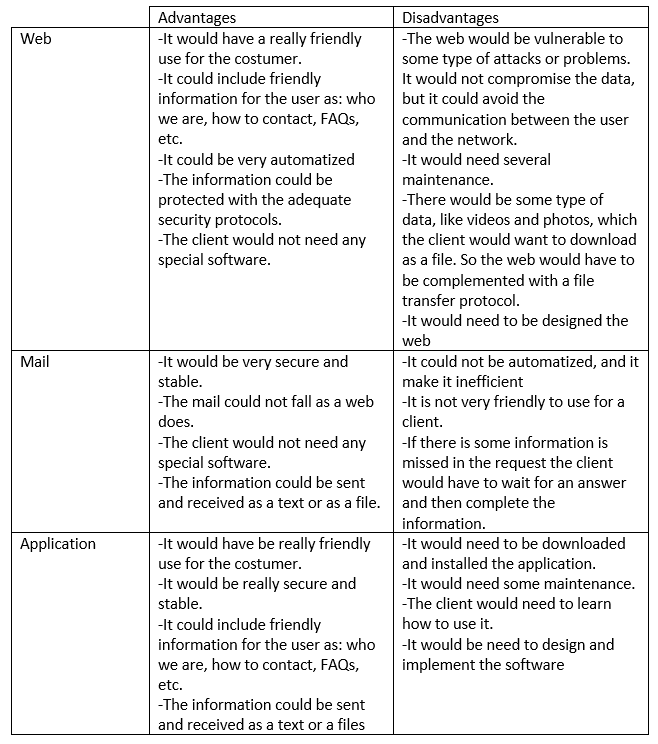
\includegraphics[scale=1]{Parts/tabla}
\end{center}

\paragraph{}
Taking in account the advantages and disadvantages of each method it is concluded that an application is the method with the better security, efficiency and frindly-use relationship. The application will ensure a high security of the data, a robust access to it, and a friendly interface for the user. More over the communication protocol that will be implemented, this system will involve the design, implementation and maintenance of the app. 
\paragraph{}
This system could work with a FTP or with a SSH. Both would work properly in the system and have very similar characteristics, but SSH is more secure than FTP, so the system would be ruled by a SSH protocol.



